\chapter{Planificación}

La planificación del proyecto es una etapa crucial que determina cómo se llevará a cabo el desarrollo del mismo, asegurando que los recursos se utilicen de manera eficiente y que se cumplan los plazos establecidos. En este capítulo, se detallará cómo se ha organizado el proyecto siguiendo los principios ágiles mencionados en el capítulo de metodología. Se describirán las herramientas y técnicas usadas para la gestión del tiempo y los recursos, así como la estructuración de las tareas en forma de \textit{issues} y \textit{milestones}.

\section{Organización del proyecto}

Como se ha mencionado anteriormente, el proyecto se organizará y planificará siguiendo un enfoque ágil. Para garantizar la aplicación coherente de estos principios, la memoria se desarrollará iterativa e incrementalmente, con actualizaciones a medida que avanza el proyecto y se toman decisiones. Esto nos permite evaluar continuamente cómo estamos añadiendo valor al proyecto.

\subsection{\textit{Issues}}

A lo largo del proyecto se van a ir encontrando diferentes problemas que se han de resolver. Para llevar un control de los mismos se han ido creando \textit{issues}. Estos no solo son descripciones de los problemas que se quieren resolver, sino que pueden ser una buena medida para saber si se progresa hacia el \textit{milestone} o no.

\begin{figure}[H]
    \caption{Captura de pantalla del listado de \textit{issues} del repositorio del proyecto de \textit{GitHub}.}
    \centering
    \vspace*{0.5cm}
    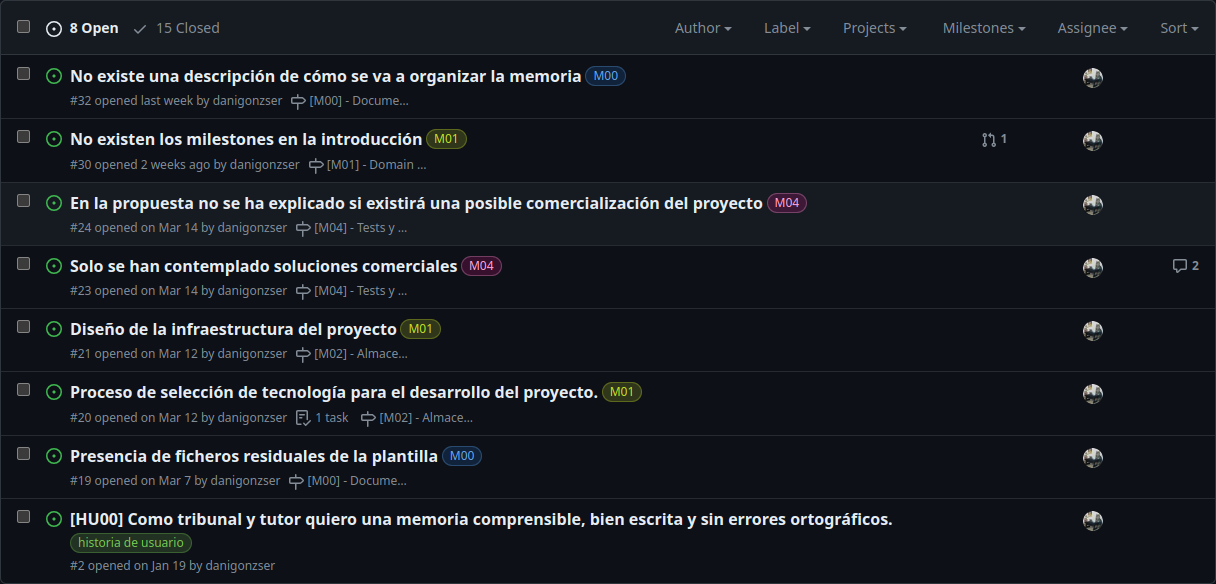
\includegraphics[scale=0.2]{figuras/github_issues.png}
\end{figure}

Existe un acceso a la documentación de la metodología seguida que se puede consultar en el siguiente \href{https://github.com/danigonzser/proyecto-tfg/issues?q=is%3Aissue+is%3Aclosed}{enlace}, aquí se encuentra el registro completo de los \textit{issues} cerrados, que ilustran el proceso de resolución de problemas y la evolución del proyecto. A continuación, se muestra un pantallazo de los \textit{issues} cerrados:

\begin{figure}[H]
    \caption{Pantallazo del listado de issues cerradas.}
    \centering
    \vspace*{0.5cm}
    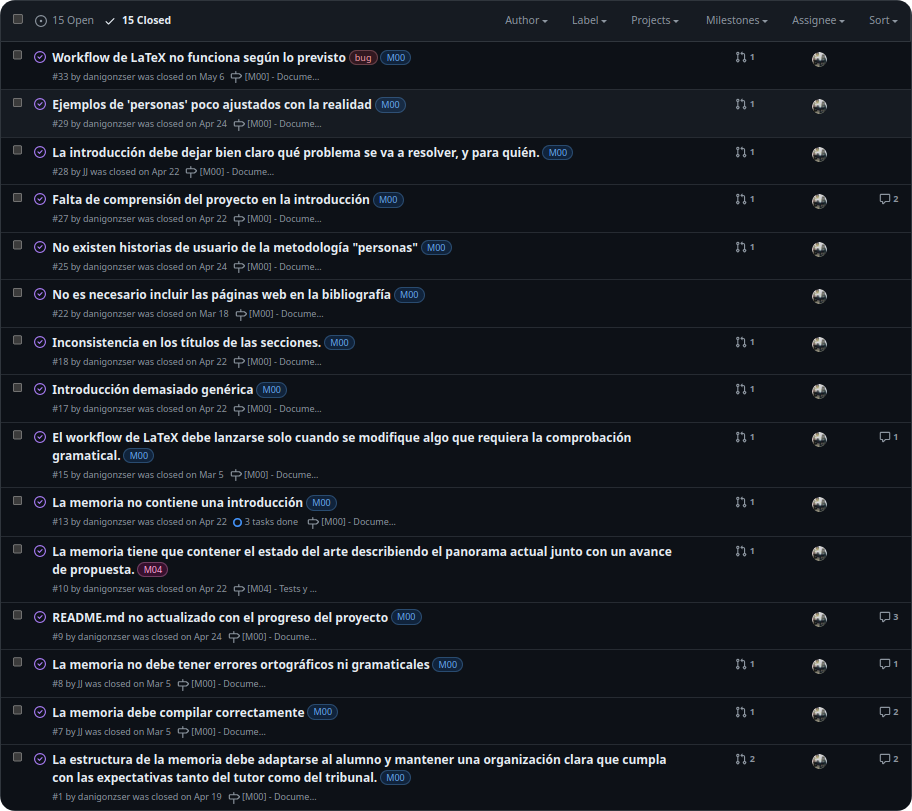
\includegraphics[scale=0.2]{figuras/listado_issues_cerradas.png}\label{fig:figuras/listado_issues_cerradas.png}
\end{figure}

\subsection{Pull requests}

Los pull requests son una manera de proponer cambios en el código fuente sin que estos se apliquen directamente al código fuente o rama principal sin una aprobación previa. Estos son una manera de revisar que los cambios mantengan la excelencia técnica y calidad del proyecto apoyando al noveno principio del manifiesto ágil.

Para proteger la rama principal o \textit{master} de cambios no deseados se han configurado una serie de reglas que impiden la integración de cambios a menos que:

\begin{itemize}
    \item Los tests deben de haberse realizado de manera exitosa.
    \item Que la rama esté actualizada.
    \item Que las conversaciones hayan sido resueltas.
\end{itemize}

A continuación se muestra una captura de pantalla de la lista de \textit{pull requests} del proyecto hasta el momento.

\begin{figure}[H]
    \caption{Captura de pantalla del listado de \textit{pull requests} del repositorio del proyecto de \textit{GitHub}.}
    \centering
    \vspace*{0.5cm}
    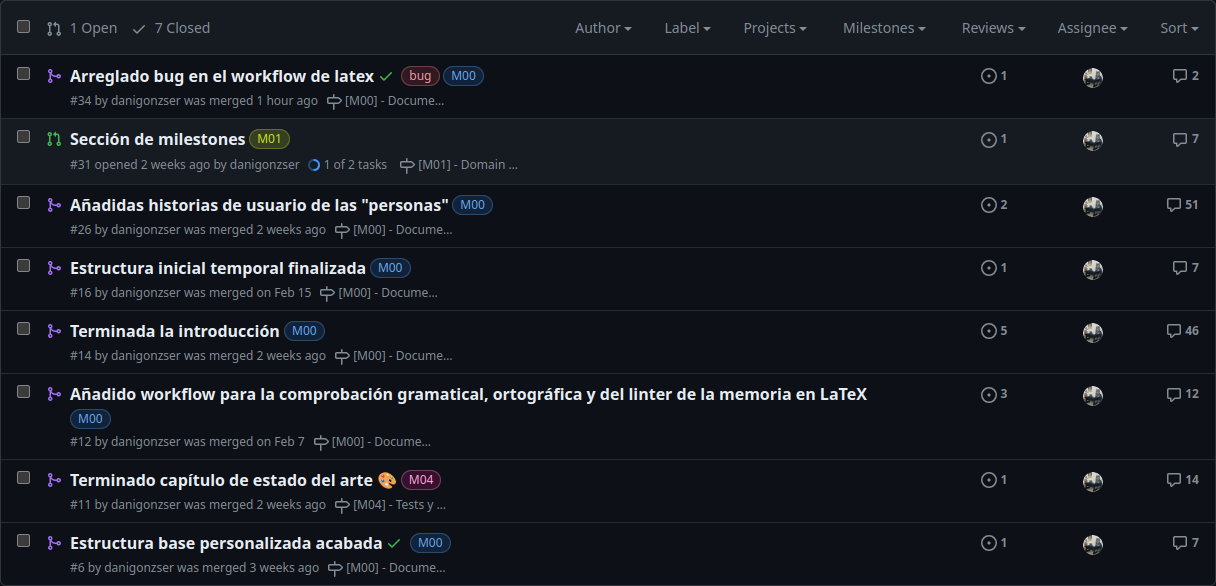
\includegraphics[scale=0.2]{figuras/listado_pull_requests_github.png}
\end{figure}

En la figura se puede apreciar que se han abierto 8 \textit{pull requests} hasta el momento. Los que están en color morado son los \textit{pull requests} que ya han sido integrados en la rama principal y el que está en color verde es el que todavía no está integrado.

\begin{figure}[H]
    \caption{Captura de pantalla del contenido de una \textit{pull request}.}
    \centering
    \vspace*{0.5cm}
    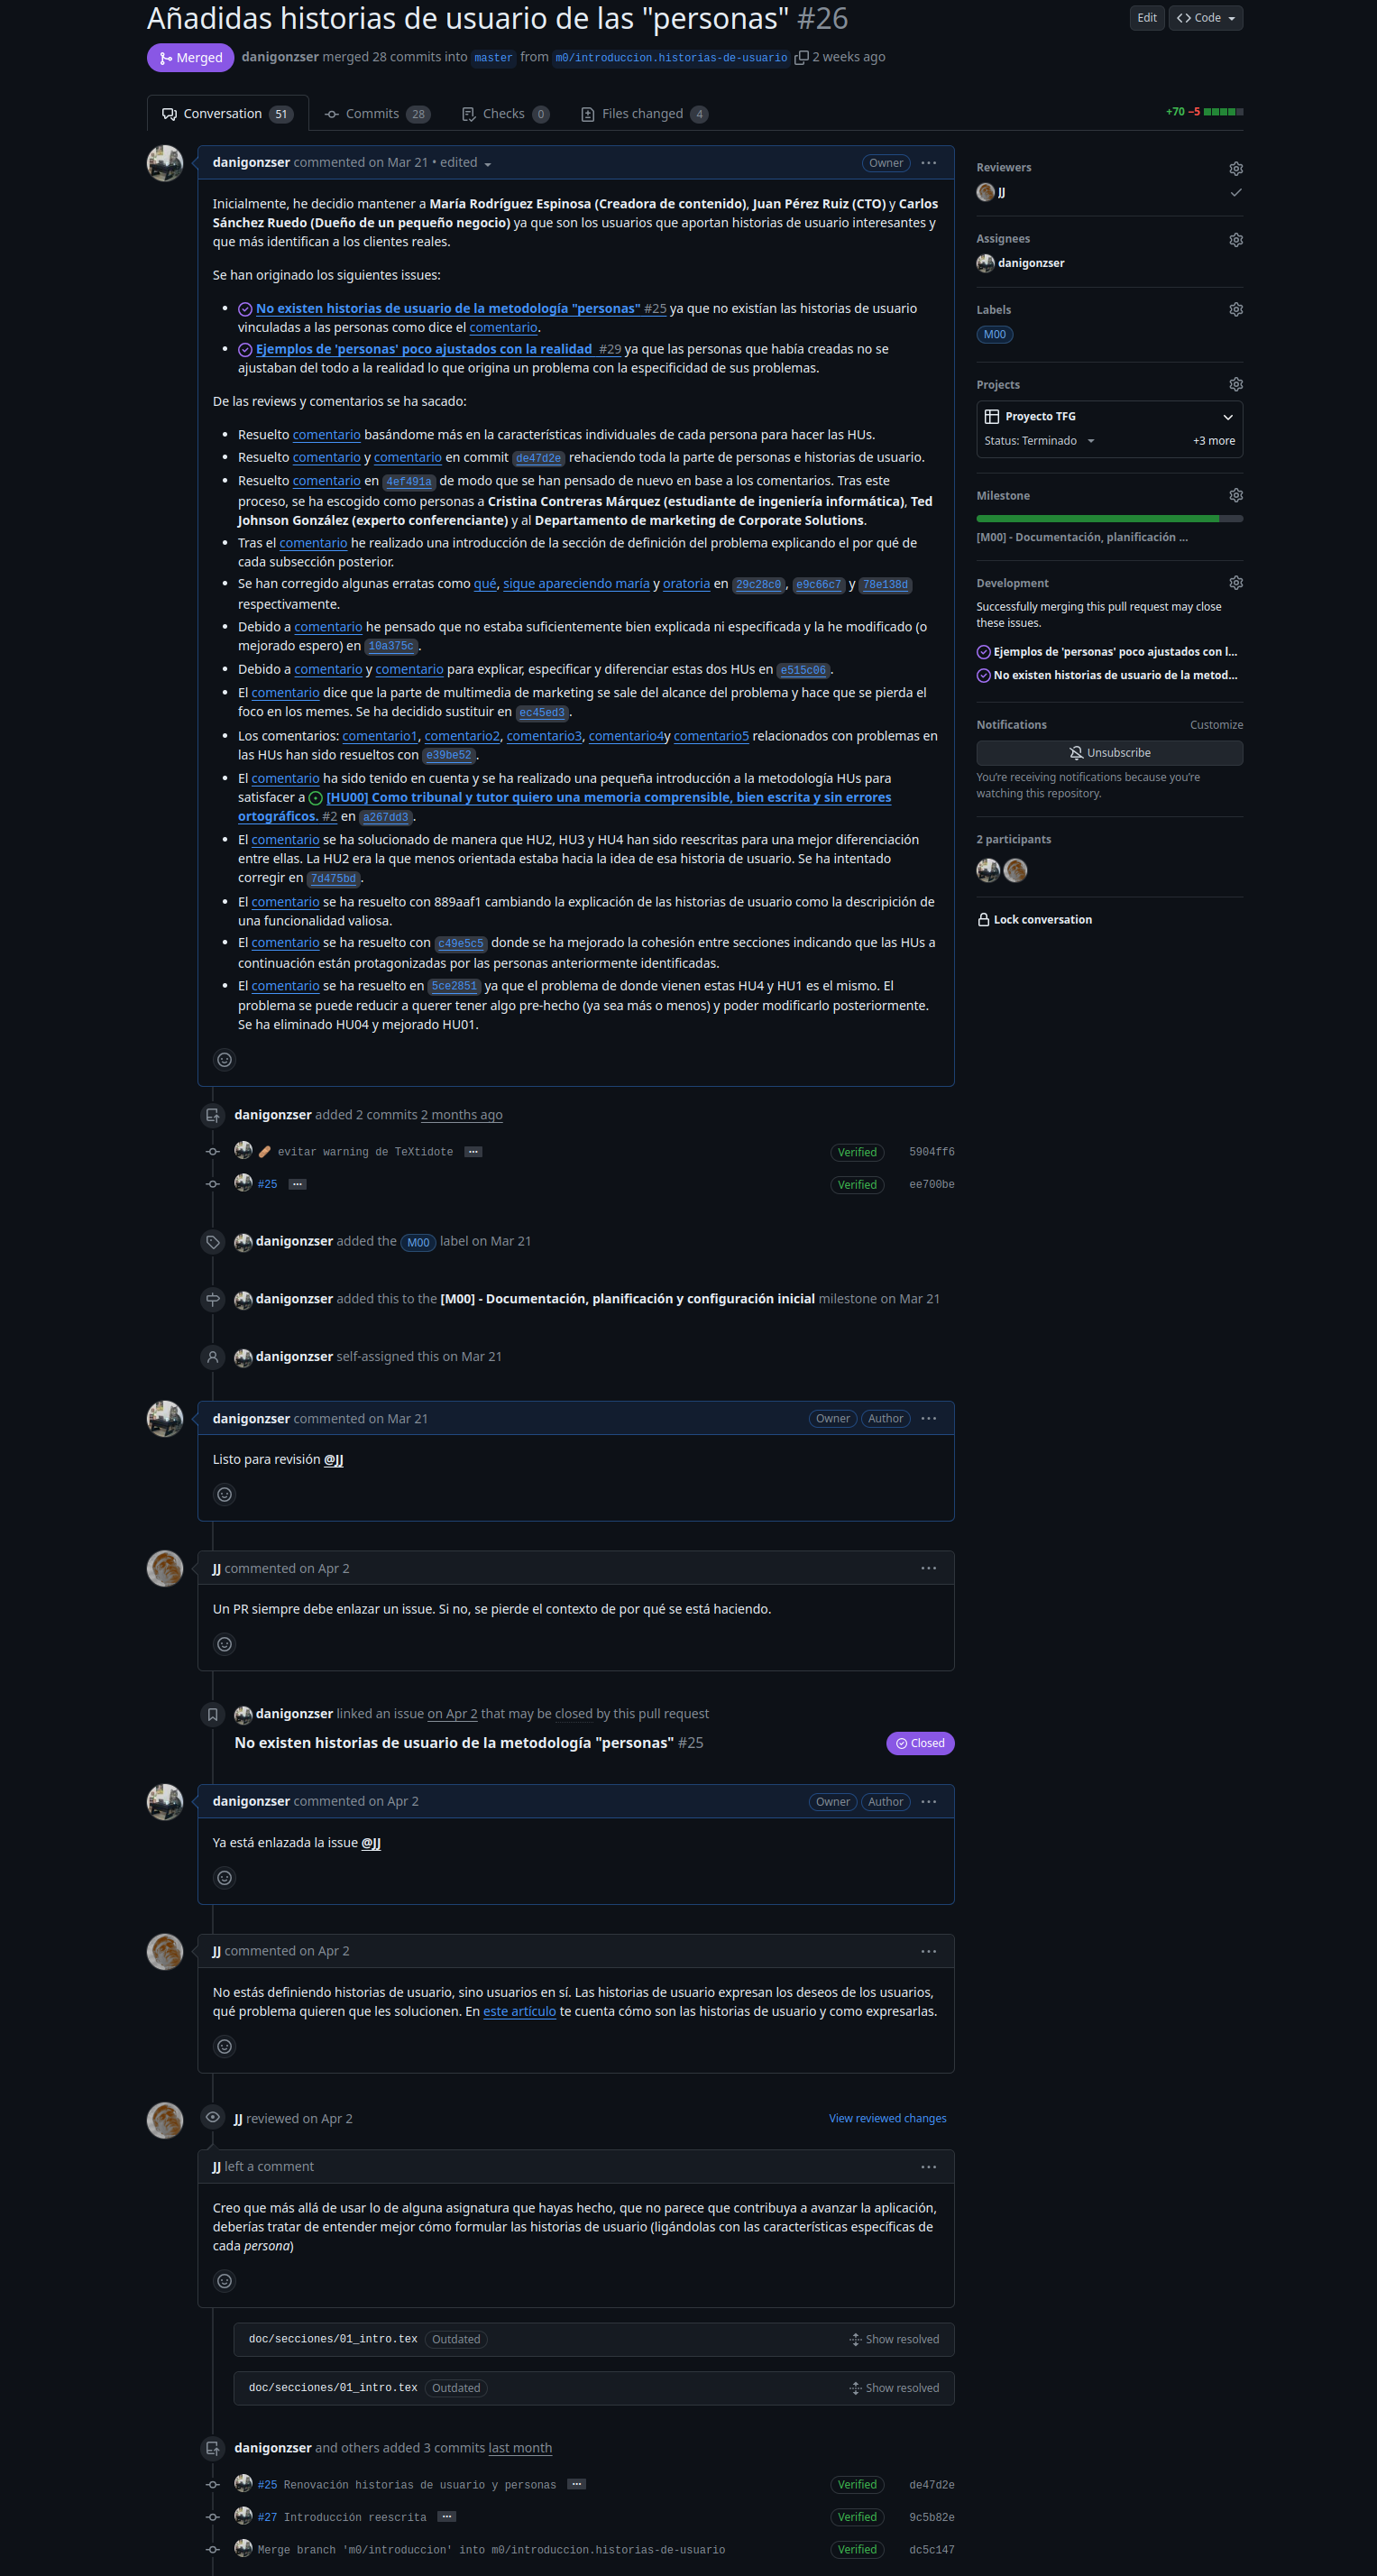
\includegraphics[scale=0.1]{figuras/pull_request_github.png}\label{fig:contenido_pull_request}
\end{figure}

Como se puede ver en la figura~\ref{fig:contenido_pull_request} el estado de la \textit{pull request} es \textit{merged} lo que significa que ya ha sido integrado en la rama principal. Más abajo se puede ver el cuerpo de la misma donde residen todas las \textit{issues} que han sido creadas y consecuentemente resueltas con esta \textit{pull request}. Más abajo se puede ver el historial de commits y de conversaciones que se han ido originando a lo largo de la resolución. Al final de la imagen es donde podemos ver esas conversaciones que deben ser resueltas antes de integrar los cambios en la rama principal. Finalmente, a la derecha se muestran detalles como el revisor, el asignado, las etiquetas, el proyecto al que pertenece, el \textit{milestone} y las \textit{issues} relacionadas.

\subsection{\textit{Projects}: tablero kanban}

La funcionalidad de projects de \textit{GitHub} se ha utilizado para llevar un control de la evolución y progreso de los \textit{issues} y \textit{pull requests}. Se ha implementado un tablero \textit{kanban} como se puede ver en la imagen~\ref{fig:tablero_kanban} que permite ver de un vistazo el estado de los \textit{issues} y \textit{pull requests}. Esto es muy útil para saber si se progresa, cómo se están resolviendo los problemas y si se está cumpliendo con los objetivos marcados. Además, está relacionado con los principios ágiles al promover la auto-organización, entrega frecuente y temprana y atención continua.

\begin{figure}[H]
    \caption{Captura de pantalla del tablero \textit{kanban} en la sección de \textit{projects} de \textit{GitHub}.}
    \centering
    \vspace*{0.5cm}
    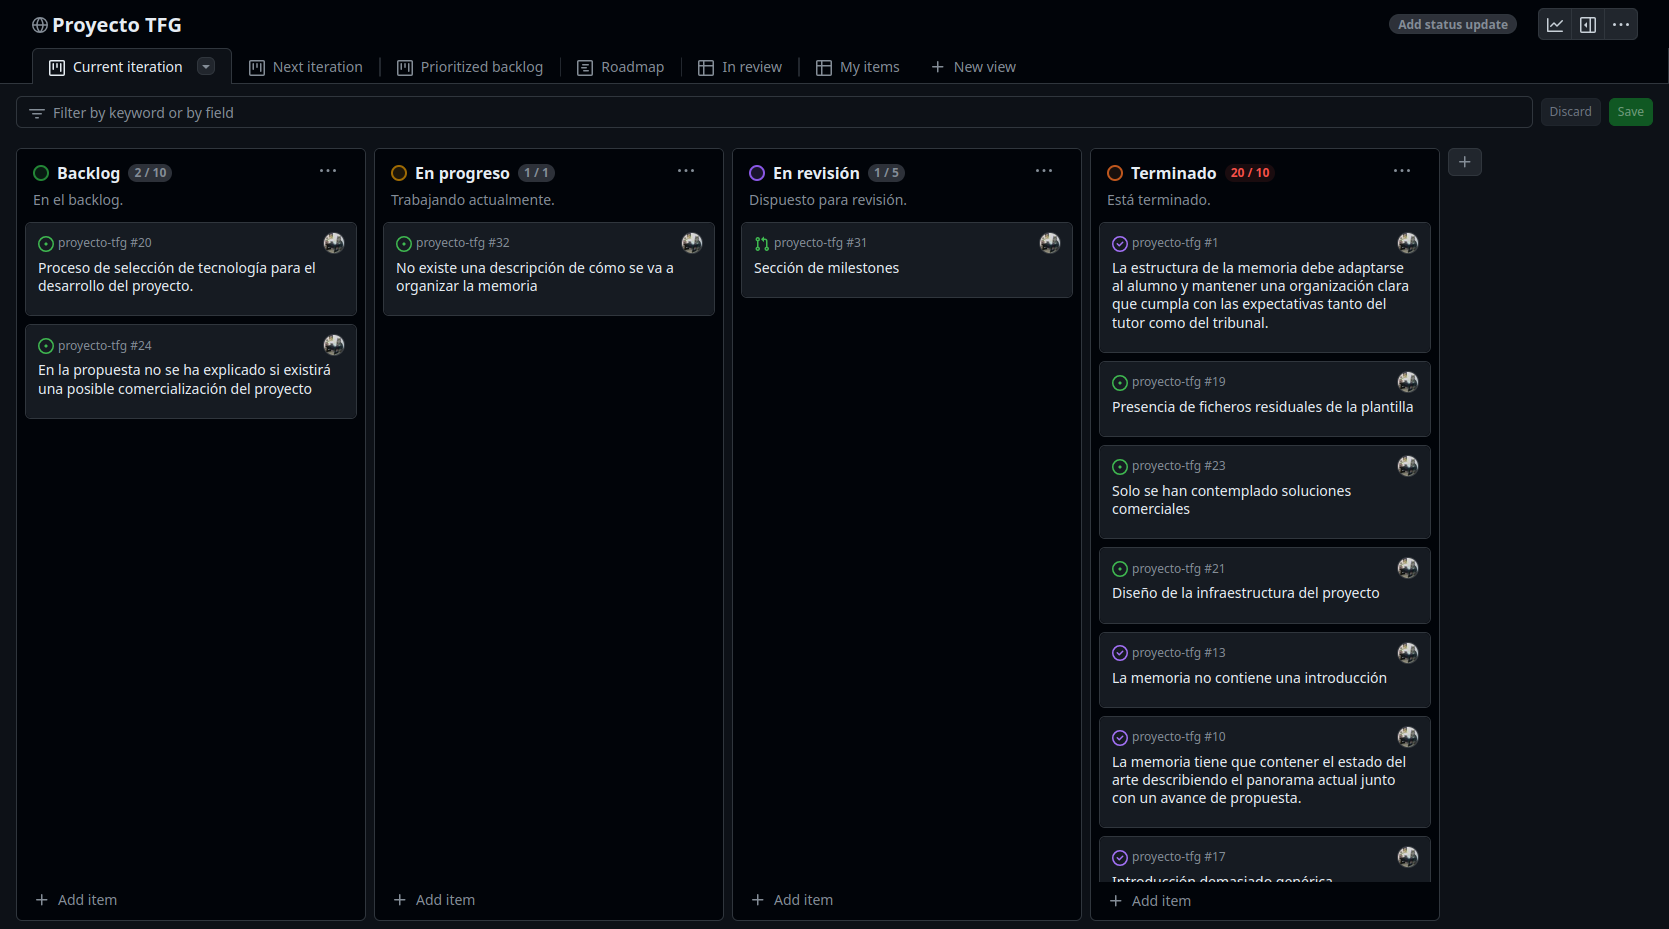
\includegraphics[scale=0.2]{figuras/projects_github.png}\label{fig:tablero_kanban}
\end{figure}

\section{Temporización}

La gestión de tiempo y recursos en nuestro proyecto se realiza mediante el uso de \textit{milestones} en GitHub, que son el equivalente a los \textit{sprints} en el enfoque ágil. Los \textit{milestones} se han creado a partir de las historias de usuario, asegurando que cada fase del proyecto esté orientada a cumplir con las necesidades y expectativas del usuario final. Un conjunto específico de \textit{issues} puede ser incluido en un \textit{milestone} y, al finalizar el \textit{sprint}, estos \textit{issues} deben estar resueltos. Al concluir el \textit{milestone}, debe resultar en un producto mínimamente viable y en nuestro repositorio vamos a etiquetarlos como nueva versión del proyecto.

\subsection{Milestones}

\begin{itemize}
    \item \textbf{[M00] \- Estructuración inicial del proyecto}
    \begin{itemize}
        \item \textit{Descripción}: Este \textit{milestone} abarca la creación de la documentación inicial, la planificación del proyecto y la configuración de las herramientas necesarias. Esta parte de la memoria inicial es esencial para establecer una base sólida para el desarrollo del proyecto, para la entrega continua y la colaboración.
    \end{itemize}

    \item \textbf{[M01] \- Modelo del dominio del problema}
    \begin{itemize}
        \item \textit{Descripción}: Mediante el DDD se va a realizar un análisis del dominio del problema. Permite obtener una comprensión profunda de todo el contexto del negocio y de la estructura del software.
    \end{itemize}
\end{itemize}

A partir de aquí, los \textit{milestones} se irán definiendo y ajustando conforme avance el proyecto, siguiendo los principios del desarrollo ágil que promueven la adaptación continua y la respuesta al cambio. Los \textit{milestones} sucesivos se centrarán en la implementación.